


\begin{center}
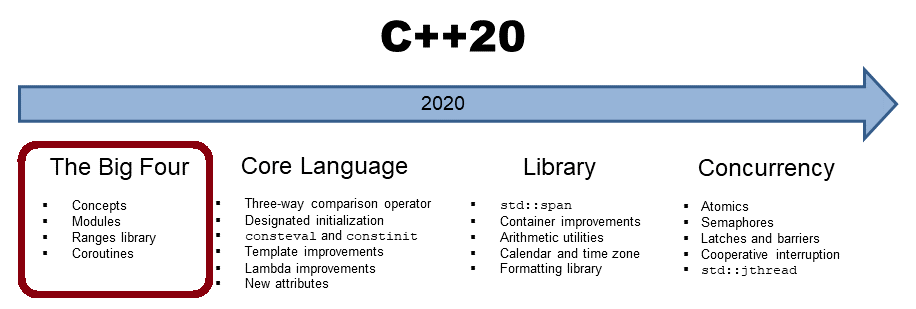
\includegraphics[width=1.0\textwidth]{content/2/chapter3/images/2.png}\\
Each feature of the Big Four changes the way we program in modern C++. Let me start with concepts.
\end{center}

\subsubsubsection{3.1.1\hspace{0.2cm}Concepts}

Generic programming with templates enables it to define functions and classes which can be used with various types. As a result, it is not uncommon that you instantiate a template with the wrong type. The result can be many pages of cryptic error messages. This problem ends with concepts. Concepts empower you to write requirements for template parameters that are checked by the compiler, and revolutionize the way we think about and write generic code. Here is why:

\begin{itemize}
\item 
Requirements for template parameters become part of their public interface.

\item 
The overloading of functions or specializations of class templates can be based on concepts.

\item 
We get improved error messages because the compiler checks the defined template parameter requirements against the given template arguments.
\end{itemize}

Additionally, this is not the end of the story.

\begin{itemize}
\item 
You can use predefined concepts or define your own.

\item 
The usage of auto and concepts is unified. Instead of auto, you can use a concept.

\item 
If a function declaration uses a concept, it automatically becomes a function template. Writing function templates is, therefore, as easy as writing a function.
\end{itemize}

The following code snippet demonstrates the definition and the use of the straightforward concept Integral:

\noindent
Definition and use of the Integral concept
\begin{lstlisting}[style=styleCXX]
template <typename T>
concept Integral = std::is_integral<T>::value;

Integral auto gcd(Integral auto a, Integral auto b) {
	if( b == 0 ) return a;
	else return gcd(b, a % b);
}
\end{lstlisting}

The Integral concept requires from its type parameter T that std::is\_integral<T>::value be true. std::is\_integral<T>::value is a value from the \href{https://en.cppreference.com/w/cpp/header/type_traits}{type traits library} checking at compile time if T is integral. If std::is\_integral<T>::value evaluates to true, all is fine; otherwise, you get a compiletime error.

The gcd algorithm determines the greatest common divisor based on the \href{https://en.wikipedia.org/wiki/Euclid}{Euclidean} algorithm. The code uses the so-called abbreviated function template syntax to define gcd. Here, gcd requires that its arguments and return type support the concept Integral. In other words, gcd is a kind of function template that puts requirements on its arguments and return value. When I remove the syntactic sugar, you can see the real nature of gcd.

Here is the semantically equivalent gcd algorithm, using a requires clause.

\noindent
Use of the concept Integral in the requires clause
\begin{lstlisting}[style=styleCXX]
template<typename T>
requires Integral<T>
T gcd(T a, T b) {
	if( b == 0 ) return a;
	else return gcd(b, a % b);
}
\end{lstlisting}

The requires clause states the requirements on the type parameters of gcd.

\subsubsubsection{3.1.2\hspace{0.2cm}Modules}

Modules promise a lot:

\begin{itemize}
\item 
Faster compile times

\item 
Reduce the need to define macros

\item 
Express the logical structure of the code

\item 
Make header files obsolete

\item 
Get rid of ugly macro workarounds
\end{itemize}

Here is the first simple math module:

\noindent
The math module
\begin{lstlisting}[style=styleCXX]
export module math;

export int add(int fir, int sec) {
  return fir + sec;
}
\end{lstlisting}

The expression export module math (line 1) is the module declaration. Putting export before the function add (line 3) exports the function. Now, it can be used by a consumer of the module.

\noindent
Use of the math module
\begin{lstlisting}[style=styleCXX]
import math;

int main() {
	add(2000, 20);
}
\end{lstlisting}

The expression import math imports the math module and makes the exported names visible in the current scope.

\subsubsubsection{3.1.3\hspace{0.2cm}The Ranges Library}

The ranges library supports algorithms which

\begin{itemize}
\item 
can operate directly on containers; you don’t need iterators to specify a range

\item 
can be evaluated lazily

\item 
can be composed
\end{itemize}

To make it short: The ranges library supports functional patterns.

The following example demonstrates function composition using the pipe symbol.

\noindent
Function composition with the pipe symbol
\begin{lstlisting}[style=styleCXX]
int main() {
	std::vector<int> ints{0, 1, 2, 3, 4, 5};
	auto even = [](int i){ return i % 2 == 0; };
	auto square = [](int i) { return i * i; };
	
	for (int i : ints | std::views::filter(even) |
						std::views::transform(square)) {
		std::cout << i << ' '; // 0 4 16
	}
}
\end{lstlisting}

Lambda expression even (line 3) is a lambda expression that returns true if an argument i is even. Lambda expression square (line 4) maps the argument i to its square. Lines 6 and 7 demonstrate function composition, which you have to read from left to right: for (int i : ints | std::views::filter(even) | std::views::transform(square)). Apply on each element of ints the even filter and map each remaining element to its square. If you are familiar with functional programming, this reads like prose.

\subsubsubsection{3.1.4\hspace{0.2cm}Coroutines}

Coroutines are generalized functions that can be suspended and resumed later while maintaining their state. Coroutines are a convenient way to write event-driven applications. Event-driven applications can be simulations, games, servers, user interfaces, or even algorithms. Coroutines are also typically used for cooperative multitasking.

C++20 does not provide concrete coroutines, instead C++20 provides a framework for implementing coroutines. This framework consists of more than 20 functions, some of which you must implement, some of which you can override. Therefore, you can tailor coroutines to your needs.

The following code snippet uses a generator to create a potentially infinite data-stream. The chapter coroutines provides the implemenation of the Generator.

\noindent
A generator for an infinite data-stream
\begin{lstlisting}[style=styleCXX]
Generator<int> getNext(int start = 0, int step = 1){
	auto value = start;
	while (true) {
		co_yield value;
		value += step;
	}
}

int main() {
	
	std::cout << '\n';
	
	std::cout << "getNext():";
	auto gen1 = getNext();
	for (int i = 0; i <= 10; ++i) {
		gen1.next();
		std::cout << " " << gen1.getValue();
	}
	
	std::cout << "\n\n";
	
	std::cout << "getNext(100, -10):";
	auto gen2 = getNext(100, -10);
	for (int i = 0; i <= 20; ++i) {
		gen2.next();
		std::cout << " " << gen2.getValue();
	}
	
	std::cout << "\n";

}
\end{lstlisting}

The function getNext is a coroutine because it uses the keyword co\_yield. There is an infinite loop which returns the value at co\_yield (line 4). A call to next (lines 16 and 25) resumes the coroutine and the following getValue call gets the value. After the getNext call returns, the coroutine pauses once again, until the next call next. There is one big unknown in this example: the return value Generator<int> of the getNext function. This is where the complication begins, which I describe in full depth in the coroutines section.

\begin{center}
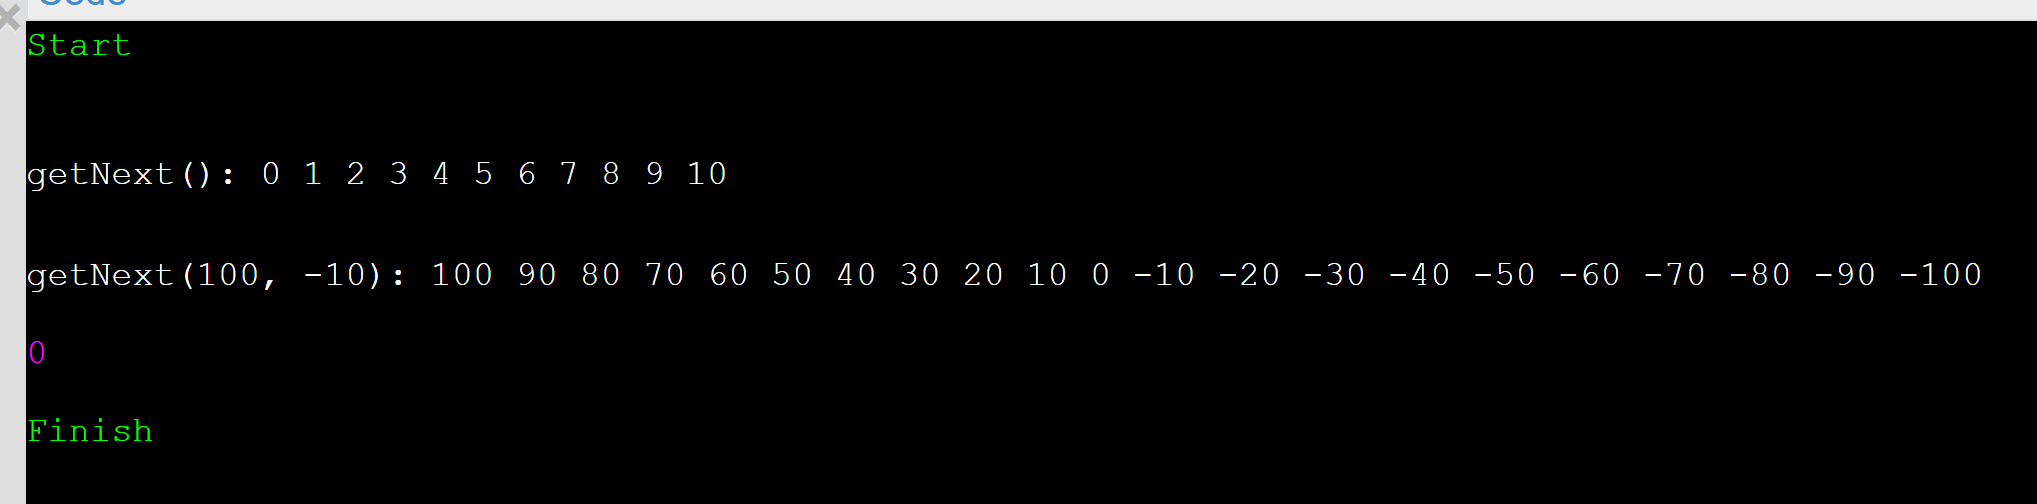
\includegraphics[width=1.0\textwidth]{content/2/chapter3/images/3.png}\\
\end{center}















